\section{Geometria}

\questao{(Elaboração própria) Qual a quantidade de quadrados (de qualquer tamanho) que você consegue identificar na figura a seguir?}

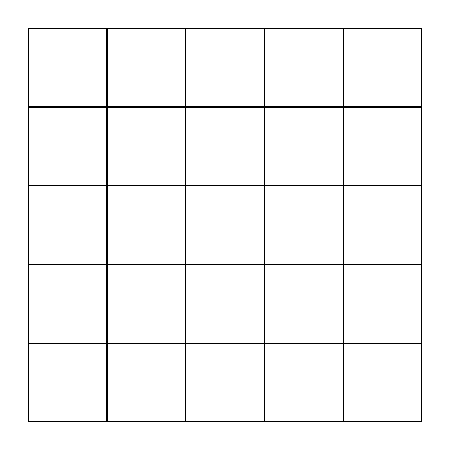
\begin{tikzpicture}
    \foreach \x in {0,1,2,3,4}{
        \foreach \y in {0,1,2,3,4}{
            \draw(\x,\y) rectangle ++(1,1);
        }
    }
\end{tikzpicture}

\begin{multicols}{4}
    \begin{enumerate}[label=\alph*)]
        \item 25
        \item 40
        \item 30
        \item 55
    \end{enumerate}
\end{multicols}

\begin{solucoes}{2}
    \solucao 

    Se considermos seguir a logica de contar cada quadrado, teremos, 25 quadradinhos 1x1, 16 quadradinhos 2x2, 9 quadrados 3x3, 4 quadrados 4x4 e 1 quadrado 5x5, assim, ficamos com a seguinte soma:

    $$25 + 16 + 9 + 4 + 1 = 55\,\, \text{Quadrados}$$

    \textbf{ALTERNATIVA D}

    \solucao

    Uma outra forma de resolver essa questão, é utilizar a formula da soma dos quadrados do enésimo termo.

    $$1^{2} + 2^{2} + 3^{2} + \cdots + n^{2} = \cfrac{n\cdot(n+1)\cdot(2n+1)}{6}$$

    Assim, ja que temos um quadrado 5x5, formado por quadradinhos 1x1, obtemos a seguinte operação:

    $$\cfrac{5\cdot(5+1)\cdot(2\cdot5+1)}{6} = \cfrac{5\cdot6\cdot11}{6} = \cfrac{5\cdot\canceldiv{6}{6}\cdot11}{\canceldiv{6}{6}} = 5\cdot11= 55 \,\, \text{quadrados totais}$$

    \textbf{ALTERNATIVA D}
\end{solucoes}